% 文件描述:这是机械结构详细设计章节中的自适应末端夹取机构部分
% 作者:耿梓行
% 上次更新:1.12.11



\section{自适应末端执行机构}

为了能够使用同一个抓手抓取不同的KFC产品,例如不同大小的汉堡、可乐、薯条等,需要夹
取机构能够适应不同的大小和形状,并且在夹取物品的同时保持其较小的形变。因而末端执行
机构采用了如下图所示的自适应设计。

\begin{figure}[!htp]
  \centering
  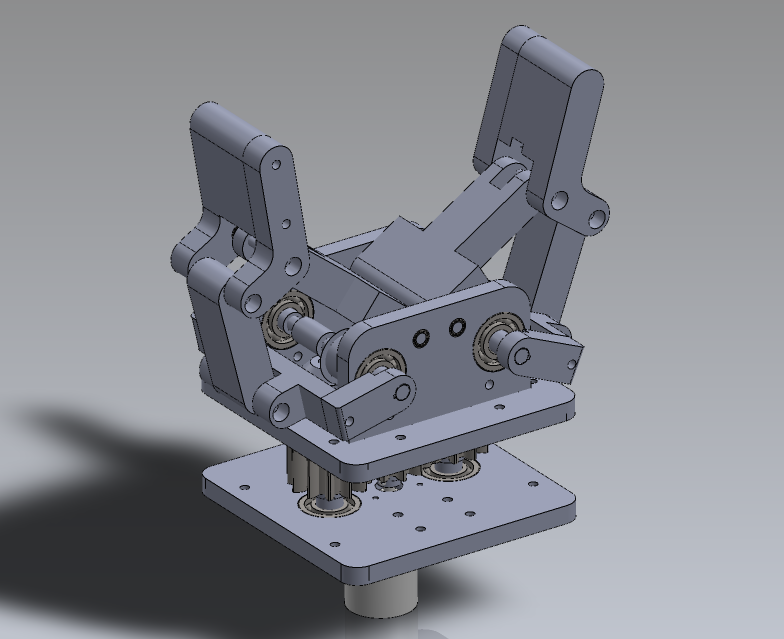
\includegraphics[width=11cm]{Overview_of_end_effectors.png} \\
  \bicaption[末端执行机构总览]
    {末端执行机构总览}
    {Overview of end actuators}
  \label{fig:末端执行机构总览}
\end{figure}

末端执行机构可以分为两个模块分别是:下层传动模块和换向夹取模块。下层传动模块负责将电机的转动
转化为伞齿轮的转动,换向夹取模块则将伞齿轮轴的转动转化为抓手的相对转动从而实现夹取动作。



\subsection{下层传动模块}

传动模块总览如图\ref{fig:下部传动模块},主要由电机、三个直齿轮、伞齿轮、轴承和上下两个机架横板组成。

\begin{figure}[!htp]
  \centering
  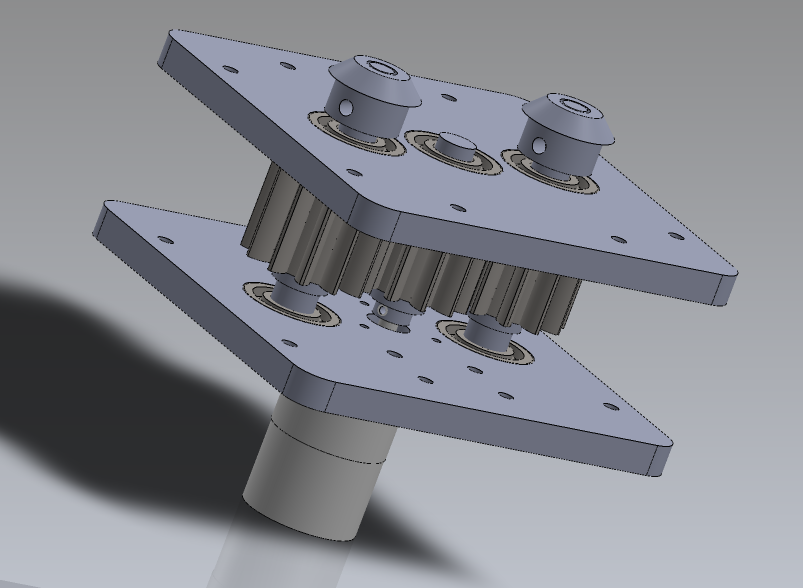
\includegraphics[width=11cm]{Lower_transmission_module.png} \\
  \bicaption[下部传动模块]
    {下部传动模块}
    {module for transmission}
  \label{fig:下部传动模块}
\end{figure}

电机通过螺钉和下机架横板固定,电机D型轴和电机外接竖轴通过紧定螺钉实现周向固定。
外接竖轴带动中间伞齿轮转动,进而通过直齿轮传动带动竖伞齿轮轴的转动。竖伞齿轮轴上部
也通过紧定螺钉和伞齿轮连接,最终使伞齿轮同向转动。
\\
\\ 
\\
\\

\subsubsection{电机外接竖轴}


\begin{figure}[!htp]
  \centering
  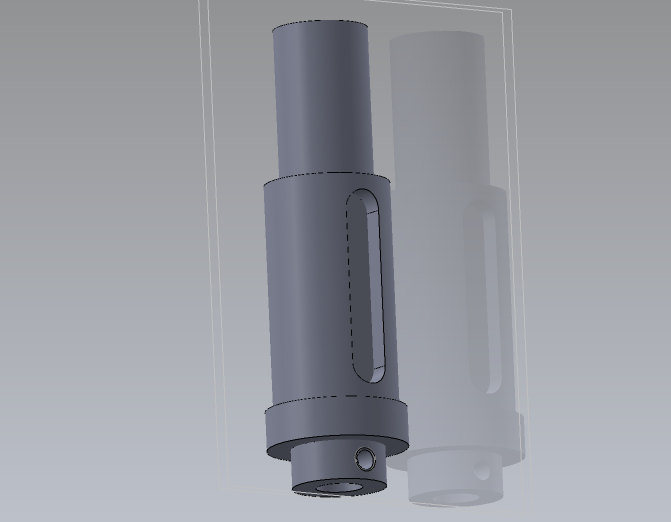
\includegraphics[width=11cm]{Motor_external_vertical_shaft.png} \\
  \bicaption[电机外接竖轴]
    {电机外接竖轴}
    {External axis of the motor}
  \label{fig:电机外接竖轴}
\end{figure}
电机外接竖轴如图\ref{fig:电机外接竖轴},轴底部开有5mm的孔和电机轴连接,侧面
开有3mm的孔用以安装紧定螺钉,轴头开键槽用以带动直齿轮转动。轴颈部分和
轴承内圈过盈配合,轴承和齿轮之间有5mm的套筒以进行轴向定位。


\subsubsection{竖伞齿轮轴}

\begin{figure}[!htp]
  \centering
  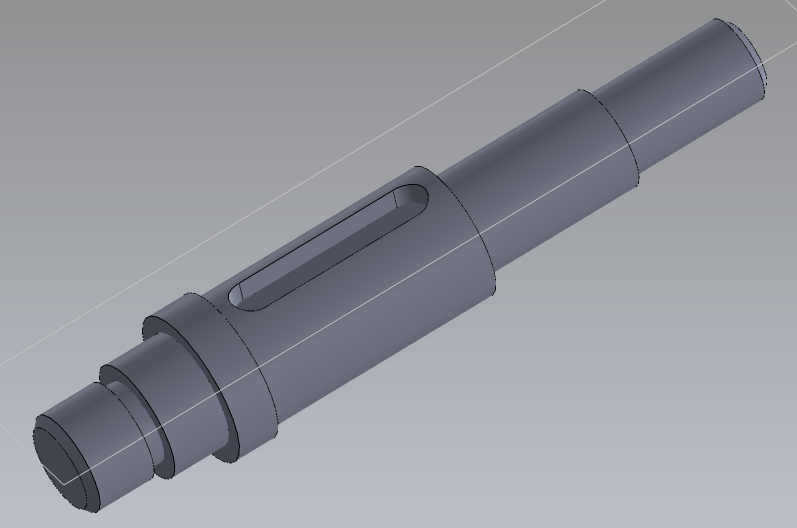
\includegraphics[width=11cm]{Shaft_gear_shaft.png} \\
  \bicaption[竖伞齿轮轴]
    {竖伞齿轮轴}
    {Vertical axis for bevel gear}
  \label{fig:竖伞齿轮轴}
\end{figure}
竖伞齿轮轴中部轴头开键槽由直齿轮带动转动。上下轴颈分别和6201深沟球轴承过盈配合
,其中下轴颈上有砂轮越程槽以方便表面磨削,直齿轮和上侧轴承由套筒轴向定位。上轴头
上装有伞齿轮,通过紧定螺钉周向定位。竖伞齿轮轴有两个,对称分布在电机外接竖轴两侧。

\subsubsection{直齿轮}

直齿轮的模数为3,内径为16mm,分度圆为36mm,齿宽为30mm,直齿轮中开键槽(查阅机械
设计手册,采用标准键槽5*5,轮毂上的深度为)。直齿轮如图\ref{fig:直齿轮} 。

\begin{figure}[!htp]
  \centering
  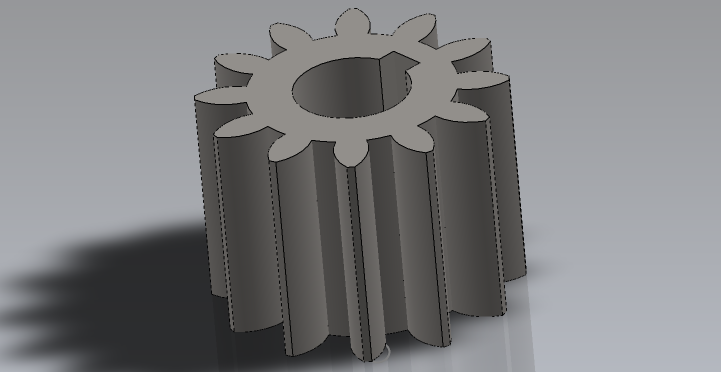
\includegraphics[width=11cm]{Spur_gear.png} \\
  \bicaption[直齿轮]
    {直齿轮}
    {Spur gear}
  \label{fig:直齿轮}
\end{figure}

\subsubsection{机架横板}

上下两个机架横板用来固定轴承,两个横板通过双头螺柱固定。其中上机架横板另打有四个
孔用以安装角铁来固定机架竖版,如图\ref{fig:上机架横板}。(机架竖版将在下一个模块介绍)
\\

\begin{figure}[!htp]
  \centering
  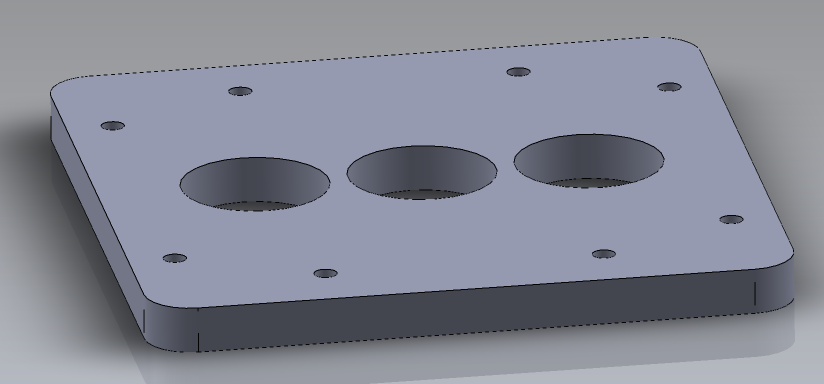
\includegraphics[width=11cm]{Upper_rack_horizontal_plate.png} \\
  \bicaption[上机架横板]
    {上机架横板}
    {Frame(upper horizontal board)}
  \label{fig:上机架横板}
\end{figure}

下机架横板中间的大圆孔直径比电机轴稍大,大孔周围的四个小孔用来固定电机,具体
结构如图\ref{fig:下机架横板}。此外,电机轴孔两侧共还有8个5mm孔用来通过螺栓
和腕部进行固定。
\\

\begin{figure}[!htp]
  \centering
  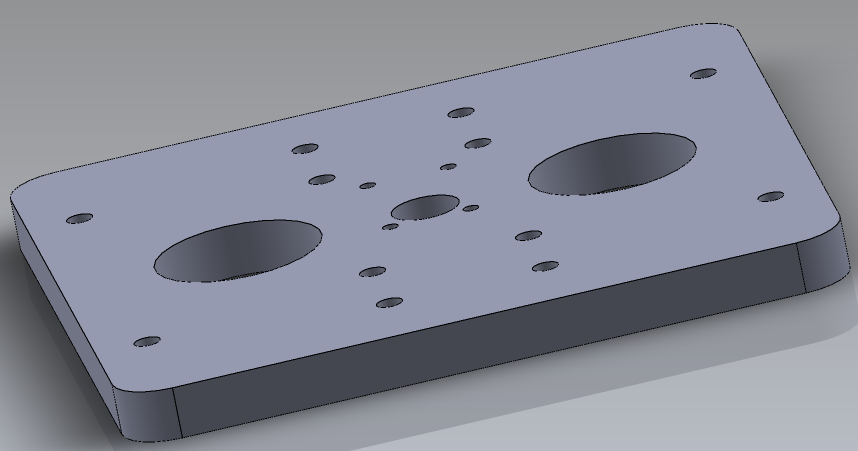
\includegraphics[width=11cm]{Under_rack_cross_plate.png} \\
  \bicaption[下机架横板]
    {下机架横板}
    {Frame(lower horizontal board)}
  \label{fig:下机架横板}
\end{figure}

\subsection{换向夹取模块}

该模块主要为了实现两部分功能:一是将竖直放置的伞齿轮的同向转动,转换为横向放置的
伞齿轮的相对转动,以使夹取物品时两抓手同时向中间靠拢;二是通过对称的两个五杆机构
和扭簧相结合实现自适应抓取。如图\ref{fig:换向夹取模块}。
\\
\\


\begin{figure}[!htp]
  \centering
  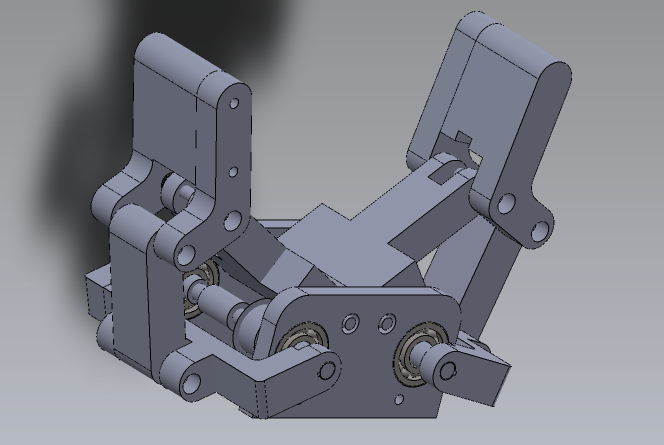
\includegraphics[width=11cm]{Reversing_clamping_module.png} \\
  \bicaption[换向夹取模块]
    {换向夹取模块}
    {Module for switching and clamping}
  \label{fig:换向夹取模块}
\end{figure}

本模块通过将水平放置的伞齿轮分别在啮合在竖直伞齿轮的对侧,实现换向功能。为了能够使
机构两侧对称,并且两侧轴承类型相同以便于加工和装配,采用两个长短不同的轴通过联轴器
连接共同构成水平伞齿轮轴。实际情况如图\ref{fig:switching}

\begin{figure}[!htp]
  \centering
  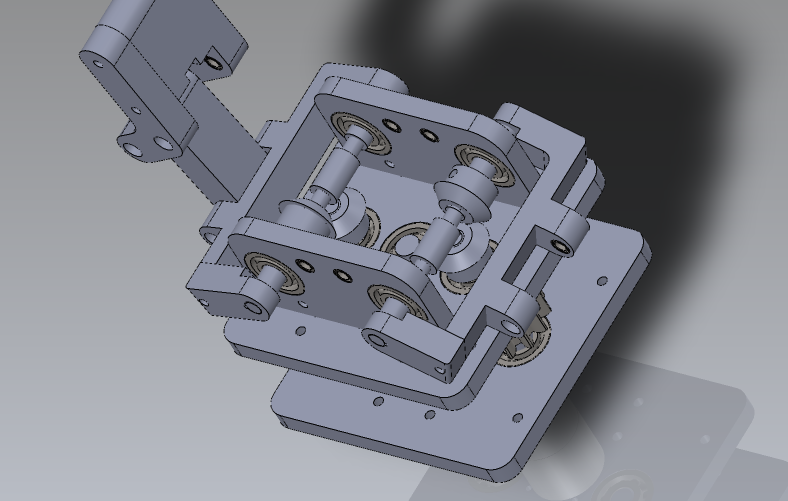
\includegraphics[width=11cm]{switching.png} \\
  \bicaption[switching]
    {换向原理图}
    {switching}
  \label{fig:switching}
\end{figure}
夹取物品通过五杆机构实现,五杆机构实际具有两个自由度,但本装置利用扭簧和被
抓物体的反作用力使抓手在夹取物品的不同阶段只具有一个自由度。扭簧套在构件3和
构件4的铰链轴上,扭簧的两脚分别和构件3与构件4固结。如图\ref{fig:五杆机构},在构件4
接触到被夹取物之前,由于扭簧的扭力的作用,构件3和构件4的相对运动会受到阻碍,此时
这两个构件近似于一个整体,相当于一个类四杆机构,构件3和构件4同时向内旋转;当构件4
接触到被夹取物时受到反作用力难以继续转动,此时杆1在水平伞齿轮轴的驱动下作为
原动件,推动构件3克服扭簧的扭力继续向内旋转。合理调整扭簧的参数就可以实现自适应的目的
构件3上装有薄膜传感器,因而可以实现对不同形状和软硬度的物品的包络和夹取,并且不会造成损坏。

\begin{figure}[!htp]
  \centering
  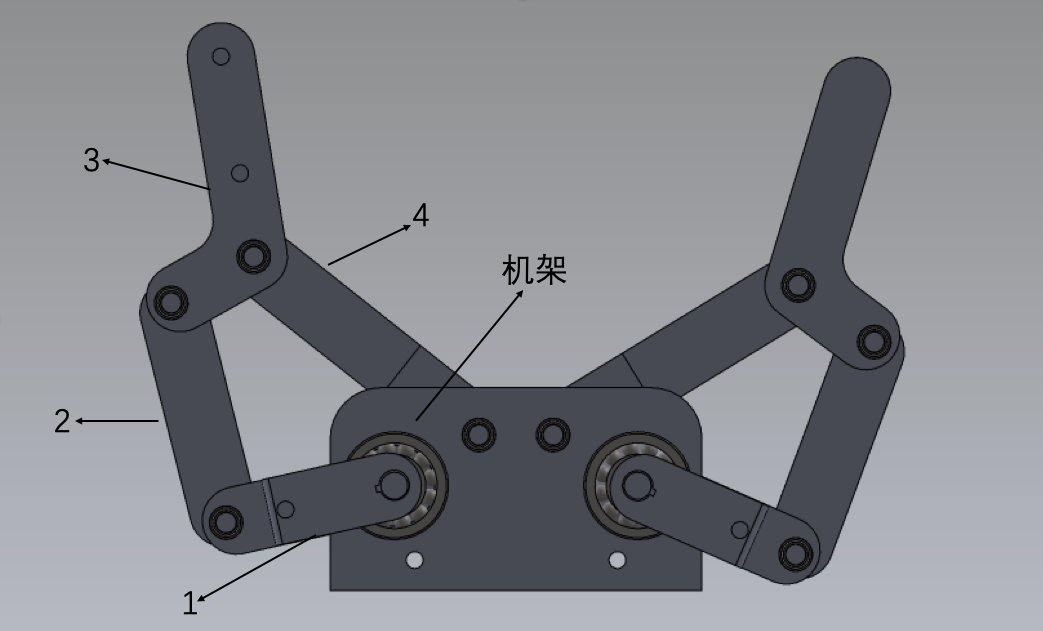
\includegraphics[width=11cm]{Five-bar_mechanism.png} \\
  \bicaption[五杆机构]
    {五杆机构}
    {five-pole mechanism}
  \label{fig:五杆机构}
\end{figure}

\subsubsection{水平伞齿轮轴}

考虑到轴承的购买和装配,以及两侧的机架竖版的加工问题,水平伞齿轮轴拟采用两部分
组成,水平伞齿轮轴1和水平伞齿轮轴2由联轴器连接,两侧轴颈部分均和6201轴承过盈配合,
两个部件如图\ref{fig:bisubcaptionbox}。

\begin{figure}[!hbtp]
  \centering
  \bisubcaptionbox{水平伞齿轮横轴1}%
                  {Horizontal axis one for the bevel gear}%
                  [6.4cm]{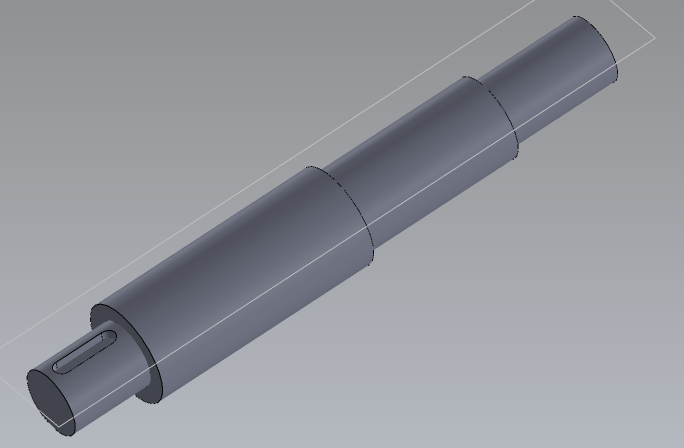
\includegraphics[height=4cm]{Horizontal_bevel_gear_shaft_1.png}}
  \hspace{1cm}
  \bisubcaptionbox{水平伞齿轮横轴2}%
                  {Horizontal axis two for the bevel gear}%
                  [6.4cm]{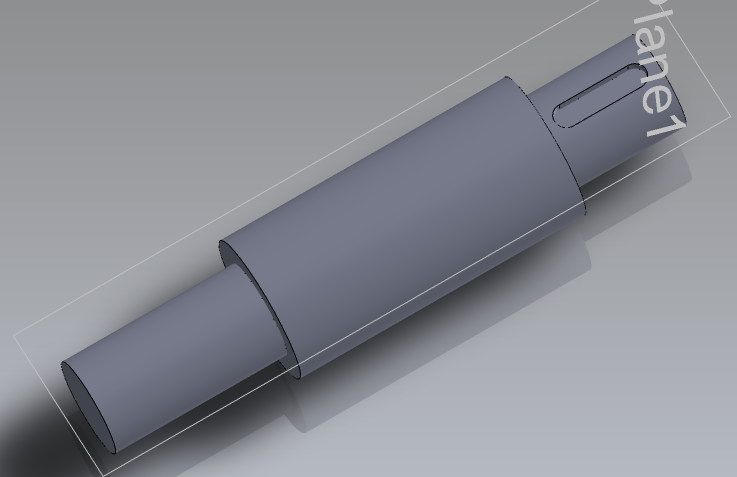
\includegraphics[height=4cm]{Horizontal_bevel_gear_shaft_2.png}}
  \bicaption{水平伞齿轮轴}
            {Example with subcaptionbox}
  \label{fig:bisubcaptionbox}
\end{figure}

水平伞齿轮轴1左下方轴头上开键槽(公称直径为2mm*2mm),用以带动五杆机构中的杆1转动,
右上第二个阶梯上装有伞齿轮并与下层传动模块上的伞齿轮啮合,无键槽的另一侧连联轴器。


水平伞齿轮轴2右上方轴头开键槽(公称直径也为2mm*2mm),中部轴颈和轴承配合,左下方与
联轴器相连。

\subsubsection{伞齿轮}
伞齿轮采用1.5模20齿,内孔为10mm,伞齿轮采用5mm的紧定螺钉固定在水平伞齿轮轴1上。
\begin{figure}[!htp]
  \centering
  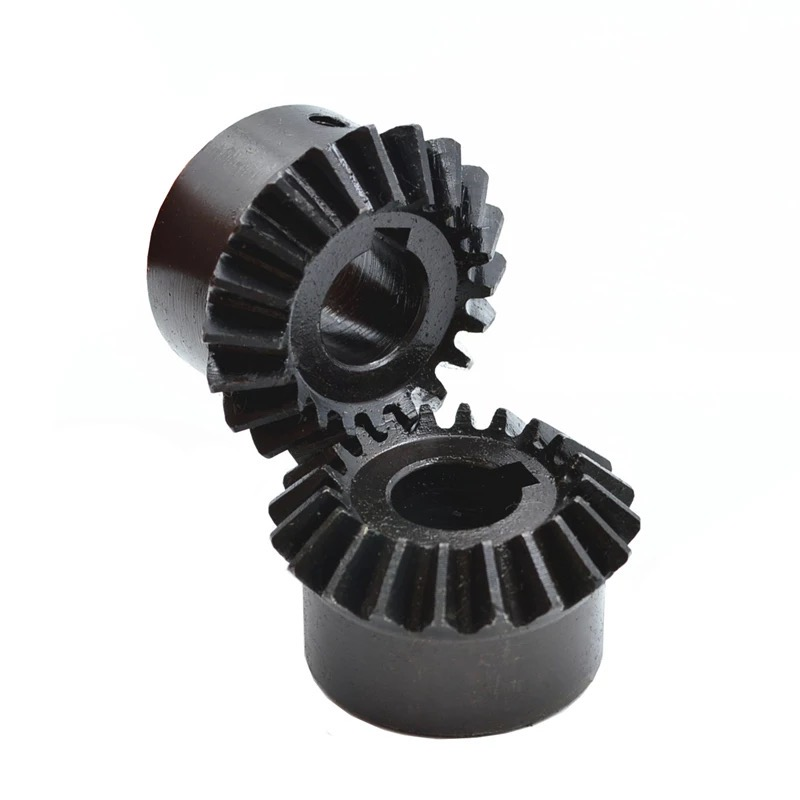
\includegraphics[width=6cm]{Bevel_gear.JPG} \\
  \bicaption[伞齿轮]
    {伞齿轮}
    {Bevel gear}
  \label{fig:伞齿轮}
\end{figure}

\subsubsection{五杆机构构件1和构件2}

构件一由两部分组成,由长螺钉固定。装配时距离较远的两个孔中有键槽,因此可以通过键链接
被水平伞齿轮轴带动;距离较近的孔通过轴承和构件2连接。构件1构件2如图\ref{fig:bisubcaptionbox}。

\begin{figure}[!hbtp]
  \centering
  \bisubcaptionbox{五杆机构构件1}%
                  {Component one}%
                  [6.4cm]{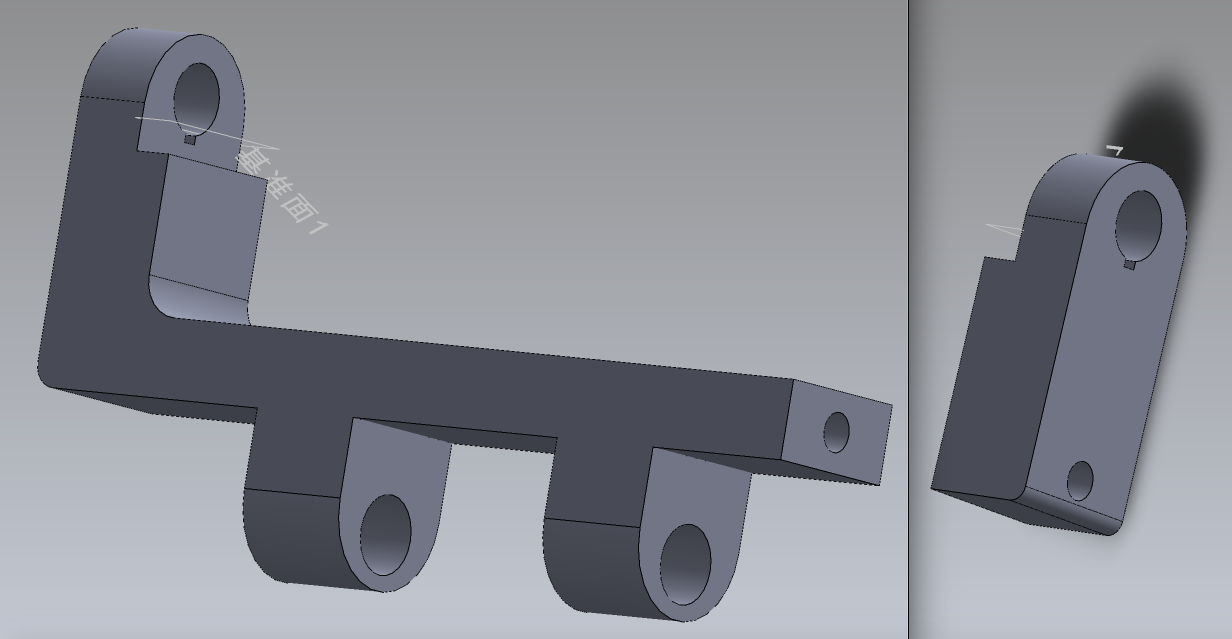
\includegraphics[height=4cm]{Five-bar_mechanism_component_1.png}}
  \hspace{1cm}
  \bisubcaptionbox{五杆机构构件2}%
                  {Component two}%
                  [6.4cm]{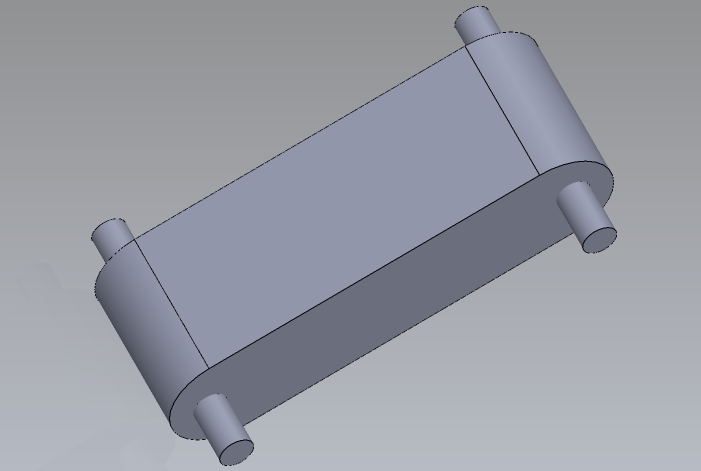
\includegraphics[height=4cm]{Five-bar_mechanism_component_2.png}}
  \bicaption{五杆机构构件1和构件2}
            {five-pole mechanism}
  \label{fig:bisubcaptionbox}
\end{figure}


\subsubsection{五杆机构构件3和构件4}

构件3也由两部分组成,通过连个螺钉连接固定。两对通孔内均装轴承,分别可夹住构件2和构件4。
构件3的主要部分上设有凹槽用来固定扭簧的一脚。

构件4设计成两部分来安装扭簧,较大的一部分上有内伸轴作为扭簧的固定轴,并且也有凹槽来固定
扭簧的另一脚。构件4的两对外伸轴分别通过轴承和构件3以及机架竖板相连。

\begin{figure}[!hbtp]
  \centering
  \bisubcaptionbox{五杆机构构件3}%
                  {Component three}%
                  [6.4cm]{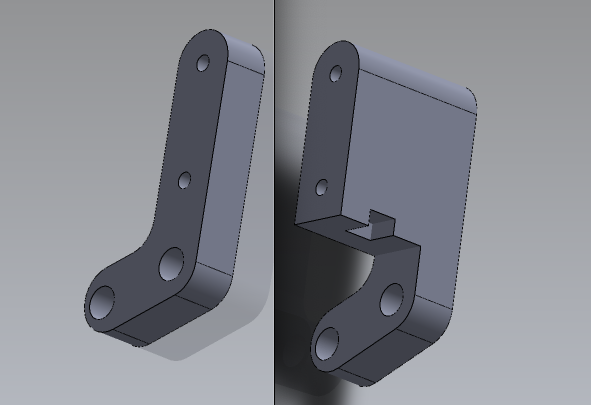
\includegraphics[height=4cm]{Five-bar_mechanism_component_3.png}}
  \hspace{1cm}
  \bisubcaptionbox{五杆机构构件4}%
                  {Component four}%
                  [6.4cm]{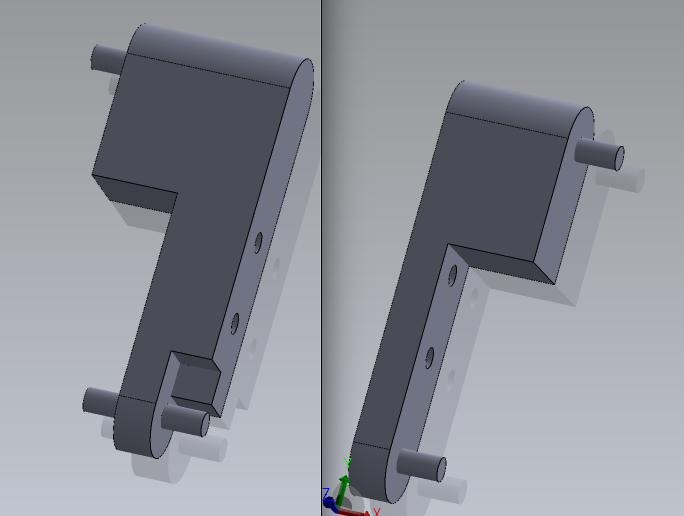
\includegraphics[height=4cm]{Five-bar_mechanism_component_4.png}}
  \bicaption{五杆机构构件3和构件4}
            {five-pole mechanism}
  \label{fig:bisubcaptionbox}
\end{figure}

\subsubsection{机架竖板}

换向夹取机构含有两个相同的机架竖板,板厚10mm,最大的一对孔用来放置6201滚动轴承,上方
小孔用来放置较小的608轴承,下方的一对小孔用来固定角铁。

\begin{figure}[!htp]
  \centering
  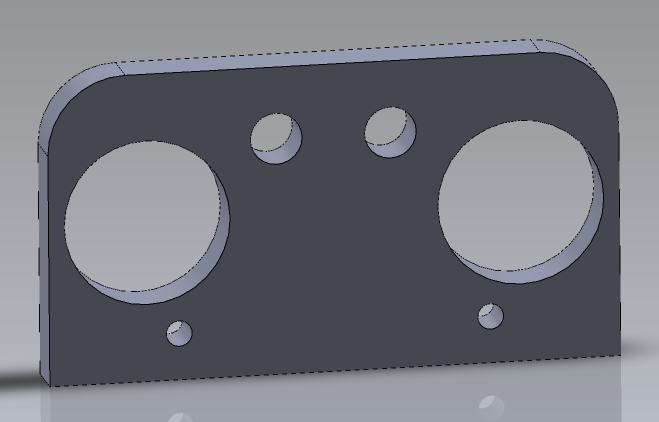
\includegraphics[width=11cm]{Rack_riser.png} \\
  \bicaption[机架竖板]
    {机架竖板}
    {Frame(vertical board)}
  \label{fig:机架竖板}
\end{figure}

\subsubsection{扭簧}

扭簧为非标准定制,扭簧线径为0.8mm,内径为6.4mm比内伸轴的直径略大以便于安装,圈数为两整圈,
材质为不锈钢,扭簧右旋。

\begin{figure}[!htp]
  \centering
  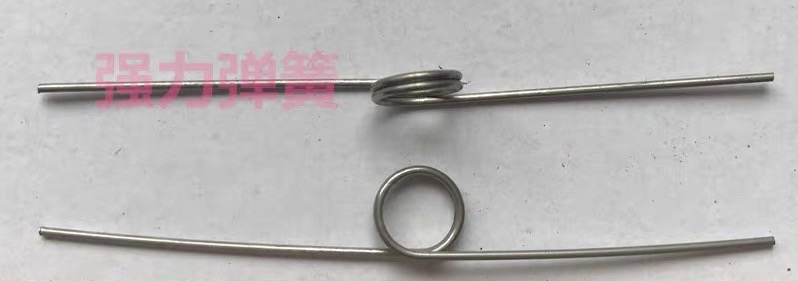
\includegraphics[width=11cm]{Torsion_spring.JPG} \\
  \bicaption[扭簧]
    {扭簧}
    {Torsion spring}
  \label{fig:扭簧}
\end{figure}

\subsection{强度校核}


\subsubsection{轴校核}
\subsubsection{直齿轮校核}
\subsubsection{伞齿轮校核}